\begin{tikzpicture}[scale=0.8]

\pgfplotstableread{
plot1   plot2   plot3   plot4
0       0       0       0
3.466   2.058   0       0
4.262   2.976   0.001   0
3.822   3.168   0.006   0.008
2.953   2.936   0.019   0.063
2.065   2.492   0.046   0.265
1.332   1.977   0.092   0.734
0.797   1.478   0.164   1.508
0.443   1.045   0.268   2.44
0.228   0.698   0.412   3.219
0.107   0.438   0.598   3.524
0.046   0.256   0.831   3.219
0.017   0.138   1.109   2.44
0.006   0.067   1.429   1.508
0.002   0.029   1.78    0.734
0       0.01    2.141   0.265
0       0.003   2.479   0.063
0       0.001   2.736   0.008
0       0       2.808   0
0       0       2.465   0
0       0       0       0
}\dummydata
\begin{axis}[
    samples=30,
    domain=-4:4,
    samples y=0, ytick={1,...,4},
    zmin=0,
    area plot/.style={
        fill opacity=0.75,
        draw=red!80!black,thick,
        fill=red,
        mark=none,
    }
]
\pgfplotsinvokeforeach{4,3,...,1}{
    \addplot3 [area plot] table [x expr=\coordindex, y expr=#1, z=plot#1]
      {\dummydata};
}
\end{axis}
\end{tikzpicture}
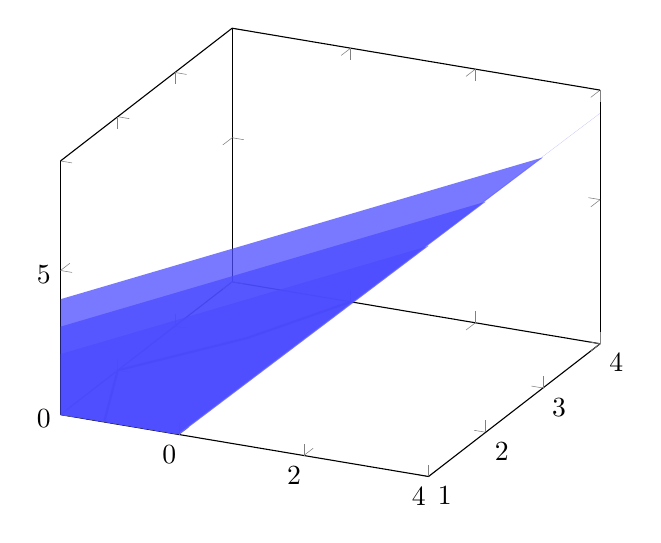
\begin{tikzpicture}[
    declare function={
        normal(\m,\s)=2*x;
    }
]
\begin{axis}[
    samples=30,
    domain=-4:4,
    samples y=0, ytick=data,
    zmin=0,
    area plot/.style={
        fill opacity=0.75,
        draw=none,
        fill=blue!70,
        mark=none,
        smooth
    }
]
\addplot3 [black, thick] table {
0 4 0
-0.75 3 0
-1.9 2 0
-1.2 1 0
};
\addplot3 [area plot] (x,4,{normal(0,1)});
\addplot3 [area plot] (x,3,{normal(-0.75,1)}) -- (axis cs:-4,3,0);
\addplot3 [area plot] (x,2,{normal(-1.9,0.7)}) -- (axis cs:-4,2,0);
\addplot3 [area plot] (x,1,{normal(-1.2,1.2)}) -- (axis cs:-4,1,0);
\end{axis}
\end{tikzpicture}
